\documentclass[11pt,a4paper]{article}
\usepackage[margin=18mm,top=22mm,bottom=20mm]{geometry}
\usepackage{fontspec}\setmainfont{Latin Modern Roman}
\usepackage{xcolor}\usepackage{amsmath,amssymb,tikz,graphicx,fancyhdr,array,needspace}
\usetikzlibrary{patterns,arrows.meta,decorations.pathmorphing,calc}
\setlength{\headheight}{14pt}
\usetikzlibrary{arrows.meta}
\pagestyle{fancy}\fancyhf{}\renewcommand{\headrulewidth}{0.4pt}
\fancyhead[L]{\textbf{M-01}}\fancyhead[C]{\itshape Fizika — yechimlar (OliyFizika.uz)}\fancyhead[R]{\textbf{Mock №1}}
\fancyfoot[C]{\thepage}
\setlength{\parindent}{0pt}\setlength{\parskip}{3pt}
\newcommand{\opt}[2]{\hspace*{4mm}#1)\ #2\par}
\newcommand{\blank}{\rule{5cm}{0.4pt}}
\begin{document}

\begin{center}{\Large\textbf{FIZIKA — YECHIMLAR}}\\[2pt]{\large Mock №1}\end{center}
\Needspace{10\baselineskip}\noindent\begin{minipage}{\linewidth}
\textbf{1.}\ Alyuminiydan yasalgan içi ğovak bölgan şar suvda 60\% qismi botgan holda suzib yuripti. Agar şarning massasi 5,4 kg ga teng bölsa, uning ğovak qismining hajmini (cm$^{3}$) toping. ($\rho_{Al}=2700$ kg/m$^{3}$)\par\smallskip
\opt{A}{5000}
\opt{B}{7000}
\opt{C}{9000}
\opt{D}{2000}
\end{minipage}\vspace{2pt}\par
\noindent\colorbox{gray!12}{\parbox{\dimexpr\linewidth-2\fboxsep}{\textbf{Javob: B) 7000}}}\par\smallskip
\noindent\textit{Yechim.}\ Şar suzganda oğirlik kuçi Arximed kuçiga teng: $\rho_s\cdot0{,}6V\,g=mg$, bundan şarning töliq hajmi\par
\[V=\frac{m}{0{,}6\rho_s}=\frac{5{,}4}{600}=9\cdot10^{-3}\ \text{m}^3=9000\ \text{cm}^3.\]
Alyuminiyning özi egallagan hajm $V_{Al}=m/\rho_{Al}=5{,}4/2700=2\cdot10^{-3}$ m$^3=2000$ cm$^3$. Ğovak hajmi $9000-2000=7000$ cm$^3$.\par\par\medskip\hrule\medskip
\Needspace{10\baselineskip}\noindent\begin{minipage}{\linewidth}
\textbf{2.}\ Jism gorizontal $X$ öqi böylab $x=2t^2-3t+2$ [m] qonunga köra harakatlanmoqda. Dastlabki 3 s da teng ta’sir etuvçi kuçning bajargan işini aniqlang (J). Jism massasi 2 kg.\par\smallskip
\opt{A}{60}
\opt{B}{72}
\opt{C}{36}
\opt{D}{108}
\end{minipage}\vspace{2pt}\par
\noindent\colorbox{gray!12}{\parbox{\dimexpr\linewidth-2\fboxsep}{\textbf{Javob: B) 72}}}\par\smallskip
\noindent\textit{Yechim.}\ Tezlik $v=x'=4t-3$: $v_0=-3$ m/s, $v(3)=9$ m/s. Kinetik energiya haqidagi teoremaga köra\par
\[A=\frac{m}{2}\left(v^2-v_0^2\right)=\frac{2}{2}(81-9)=72\ \text{J}.\]\par\medskip\hrule\medskip
\Needspace{10\baselineskip}\noindent\begin{minipage}{\linewidth}
\textbf{3.}\ Bambukning ziçligi 400 kg/m$^{3}$. Bambukli solning qalinligi 0,5 m, yuzasi 10 m$^{2}$ bölsa, unda köpi bilan neça tonna yuk taşiş mumkin?\par\smallskip
\opt{A}{2}
\opt{B}{5}
\opt{C}{3}
\opt{D}{2,5}
\end{minipage}\vspace{2pt}\par
\noindent\colorbox{gray!12}{\parbox{\dimexpr\linewidth-2\fboxsep}{\textbf{Javob: C) 3}}}\par\smallskip
\noindent\textit{Yechim.}\ Solning hajmi $V=Sh=10\cdot0{,}5=5$ m$^3$, massasi $m=400\cdot5=2000$ kg. Sol töliq botganda Arximed kuçi $\rho_s Vg$ ga teng, ya’ni $5000$ kg massali jism oğirligini kötaradi. Yuk massasi $M=5000-2000=3000$ kg $=3$ t.\par\par\medskip\hrule\medskip
\Needspace{10\baselineskip}\noindent\begin{minipage}{\linewidth}
\textbf{4.}\ Radiusi 20 cm, burçak tezligi 0,5 rad/s bölgan disk çekka nuqtasining çiziqli tezligini (m/s) toping.\par\smallskip
\opt{A}{1}
\opt{B}{0,1}
\opt{C}{0,6}
\opt{D}{0,3}
\end{minipage}\vspace{2pt}\par
\noindent\colorbox{gray!12}{\parbox{\dimexpr\linewidth-2\fboxsep}{\textbf{Javob: B) 0,1}}}\par\smallskip
\noindent\textit{Yechim.}\ $v=\omega R=0{,}5\cdot0{,}2=0{,}1$ m/s.\par\par\medskip\hrule\medskip
\Needspace{10\baselineskip}\noindent\begin{minipage}{\linewidth}
\textbf{5.}\ Moddiy nuqta vertikal yönalişda 3 s, gorizontal yönalişda 4 s davr bilan garmonik tebranmoqda. $t$=5 s paytda nuqta muvozanat nuqtasidan ötgan bölsa, yana qaysi eng yaqin $t$ paytda (s) nuqta muvozanat nuqtasiga qaytib keladi?\par\smallskip
\opt{A}{12}
\opt{B}{17}
\opt{C}{6}
\opt{D}{11}
\end{minipage}\vspace{2pt}\par
\noindent\colorbox{gray!12}{\parbox{\dimexpr\linewidth-2\fboxsep}{\textbf{Javob: D) 11}}}\par\smallskip
\noindent\textit{Yechim.}\ Nuqta muvozanat holatidan ötişi uçun ikkala tebraniş ham bir vaqtda muvozanatdan ötişi kerak. Vertikal tebraniş har $T_1/2=1{,}5$ s da, gorizontal tebraniş har $T_2/2=2$ s da muvozanatdan ötadi. Ikkalasi uçun umumiy eng kiçik vaqt $\mathrm{EKUK}(1{,}5;\,2)=6$ s. Demak, $t=5+6=11$ s.\par\par\medskip\hrule\medskip
\Needspace{10\baselineskip}\noindent\begin{minipage}{\linewidth}
\textbf{6.}\ Detalni defektoskop yordamida ultratovuşli tekşiruvdan ötkazganda detal sirtidan 10 cm çuqurligida kovak borligi aniqlandi. Agar ultratovuş signalining nuqsondan akslaniş (signalning borib keliş vaqti) vaqti 50 $\mu$s ga teng bölsa, tovuşning detal içida tarqaliş tezligini toping (m/s).\par\smallskip
\opt{A}{5000}
\opt{B}{8000}
\opt{C}{3000}
\opt{D}{4000}
\end{minipage}\vspace{2pt}\par
\noindent\colorbox{gray!12}{\parbox{\dimexpr\linewidth-2\fboxsep}{\textbf{Javob: D) 4000}}}\par\smallskip
\noindent\textit{Yechim.}\ Signal kovakkaça borib qaytadi: $2h=vt$,\par
\[v=\frac{2h}{t}=\frac{2\cdot0{,}1}{50\cdot10^{-6}}=4000\ \text{m/s}.\]\par\medskip\hrule\medskip
\Needspace{10\baselineskip}\noindent\begin{minipage}{\linewidth}
\textbf{7.}\ 600 şimoliy kenglik çiziği böylab Grinviçdan şarqqa tomon uçayotgan samolyot şarqiy uzunlik böyiça 100 da va 1000 da joylaşgan meridian çiziqlari orasini qança vaqtda ötadi (soat)? Samolyot tezligi 314 km/h. Yer radiusi 6400 km.\par\smallskip
\opt{A}{24}
\opt{B}{16}
\opt{C}{32}
\opt{D}{64}
\end{minipage}\vspace{2pt}\par
\noindent\colorbox{gray!12}{\parbox{\dimexpr\linewidth-2\fboxsep}{\textbf{Javob: B) 16}}}\par\smallskip
\noindent\textit{Yechim.}\ $60^\circ$ kenglikdagi parallel radiusi $r=R\cos60^\circ=3200$ km. $10^\circ$ va $100^\circ$ meridianlar orasidagi yoy $90^\circ$, ya’ni aylananing çoragi:\par
\[s=\frac{2\pi r}{4}=\frac{2\cdot3{,}14\cdot3200}{4}=5024\ \text{km},\qquad t=\frac{s}{v}=\frac{5024}{314}=16\ \text{soat}.\]\par\medskip\hrule\medskip
\Needspace{10\baselineskip}\noindent\begin{minipage}{\linewidth}
\textbf{8.}\ 80 kg massali odam köldan suzib ötiş uçun sol yasamoqçi. Agar solning qalinligi 20 cm bölsa, uning yuzasi (m$^{2}$) kamida qança bölişi kerak? Sol tayyorlanadigan yoğoçning ziçligi 600 kg/m$^{3}$, $\rho_{suv}$=1000 kg/m$^{3}$\par\smallskip
\opt{A}{1}
\opt{B}{1,4}
\opt{C}{0,8}
\opt{D}{1,2}
\end{minipage}\vspace{2pt}\par
\noindent\colorbox{gray!12}{\parbox{\dimexpr\linewidth-2\fboxsep}{\textbf{Javob: A) 1}}}\par\smallskip
\noindent\textit{Yechim.}\ Sol töliq botgan holda odamni kötarişi kerak: $\rho_s Shg=\rho Shg+Mg$, bundan\par
\[S=\frac{M}{(\rho_s-\rho)h}=\frac{80}{400\cdot0{,}2}=1\ \text{m}^2.\]\par\medskip\hrule\medskip
\Needspace{10\baselineskip}\noindent\begin{minipage}{\linewidth}
\textbf{9.}\ Gorizontal yölda tekis tezlanuvçan harakatlanayotgan aravaça ustida ğişt turibdi. Agar ğişt va arava orasidagi işqalaniş koeffitsiyenti 0,5 ga teng bölsa, aravaning qanday qiymatli tezlanişigaça ğişt aravadan sirpanib tuşmaydi (m/s$^{2}$)? g=10 N/kg.\par\smallskip
\opt{A}{3}
\opt{B}{5}
\opt{C}{6}
\opt{D}{4}
\end{minipage}\vspace{2pt}\par
\noindent\colorbox{gray!12}{\parbox{\dimexpr\linewidth-2\fboxsep}{\textbf{Javob: B) 5}}}\par\smallskip
\noindent\textit{Yechim.}\ Ğiştga tezlaniş faqat tinçlikdagi işqalaniş kuçi beradi: $ma\le\mu mg$, demak $a_{max}=\mu g=0{,}5\cdot10=5$ m/s$^2$.\par\par\medskip\hrule\medskip
\Needspace{10\baselineskip}\noindent\begin{minipage}{\linewidth}
\textbf{10.}\ Daryodan olingan S masofani kater oqimga qarşi suzganda 4 soatda, oqim böylab suzganda 2 soatda bosib ötadi. Agar turğun suvdagi tezligi bu katerning turğun suvdagi tezligidan 2 marta katta bölgan boşqa kater jönatilsa, bu masofani oqim böylab suzsa qança vaqtda (h) bosib ötadi?\par\smallskip
\opt{A}{3/2}
\opt{B}{6/5}
\opt{C}{1}
\opt{D}{8/7}
\end{minipage}\vspace{2pt}\par
\noindent\colorbox{gray!12}{\parbox{\dimexpr\linewidth-2\fboxsep}{\textbf{Javob: D) 8/7}}}\par\smallskip
\noindent\textit{Yechim.}\ Kater tezligi $v$, oqim tezligi $u$: $v-u=S/4$, $v+u=S/2$. Bundan $v=3S/8$, $u=S/8$. Ikkinçi kater tezligi $2v=3S/4$, oqim böylab\par
\[t=\frac{S}{2v+u}=\frac{S}{3S/4+S/8}=\frac{8}{7}\ \text{h}.\]\par\medskip\hrule\medskip
\Needspace{10\baselineskip}\noindent\begin{minipage}{\linewidth}
\textbf{11.}\ Moddalarda böladigan issiqlik hodisalarini va bu moddalarning içki xossalarini barça moddalar tartibsiz harakat qiluvçi va özaro ta’sirlaşuvçi zarralardan iboratdir, degan tasavvur asosida tuşuntiradigan nazariya... nazariya deb ataladi.\par\smallskip
\opt{A}{termodinamik}
\opt{B}{issiqlik}
\opt{C}{molekulyar-kinetik}
\opt{D}{kvant}
\end{minipage}\vspace{2pt}\par
\noindent\colorbox{gray!12}{\parbox{\dimexpr\linewidth-2\fboxsep}{\textbf{Javob: C) molekulyar-kinetik}}}\par\smallskip
\noindent\textit{Yechim.}\ Ta’rif böyiça bu — molekulyar-kinetik nazariya.\par\par\medskip\hrule\medskip
\Needspace{10\baselineskip}\noindent\begin{minipage}{\linewidth}
\textbf{12.}\ Siğimi 831 cm$^{3}$ bölgan idişda 300 K haroratli 2 g vodorod bor. Gazning bosimini aniqlang (MPa).\par\smallskip
\opt{A}{3}
\opt{B}{4}
\opt{C}{2}
\opt{D}{1}
\end{minipage}\vspace{2pt}\par
\noindent\colorbox{gray!12}{\parbox{\dimexpr\linewidth-2\fboxsep}{\textbf{Javob: A) 3}}}\par\smallskip
\noindent\textit{Yechim.}\ Mendeleyev–Klapeyron tenglamasidan ($M_{H_2}=2$ g/mol):\par
\[p=\frac{mRT}{MV}=\frac{1\cdot8{,}31\cdot300}{831\cdot10^{-6}}=3\cdot10^{6}\ \text{Pa}=3\ \text{MPa}.\]\par\medskip\hrule\medskip
\Needspace{10\baselineskip}\noindent\begin{minipage}{\linewidth}
\textbf{13.}\ Xonada elektr peçkasini L qöşilgandan söng havoning harorat 18 $^\circ$C dan 27 $^\circ$C gaça oşganligi va xonadagi havoning bosim özgarmaganligi ma’lum bölsa, xonadagi havo molekulalarining soni neça foizga kamayganini aniqlang.\par\smallskip
\opt{A}{3}
\opt{B}{9}
\opt{C}{6}
\opt{D}{1,5}
\end{minipage}\vspace{2pt}\par
\noindent\colorbox{gray!12}{\parbox{\dimexpr\linewidth-2\fboxsep}{\textbf{Javob: A) 3}}}\par\smallskip
\noindent\textit{Yechim.}\ $p$ va $V$ özgarmas bölgani uçun $N=pV/(kT)\sim1/T$:\par
\[\frac{N_2}{N_1}=\frac{T_1}{T_2}=\frac{291}{300}=0{,}97,\]
ya’ni molekulalar soni $3\%$ ga kamaygan.\par\par\medskip\hrule\medskip
\Needspace{10\baselineskip}\noindent\begin{minipage}{\linewidth}
\textbf{14.}\ Quyidagi tenglamalar içidan izobarik jarayon (Gey-Lyussak qonuni) tenglamasini toping.\par\smallskip
\opt{A}{$p_1V_1=p_2V_2$}
\opt{B}{$p=\dfrac23nE_k$}
\opt{C}{$pV=\dfrac{m}{M}RT$}
\opt{D}{$\dfrac{V_1}{T_1}=\dfrac{V_2}{T_2}$}
\end{minipage}\vspace{2pt}\par
\noindent\colorbox{gray!12}{\parbox{\dimexpr\linewidth-2\fboxsep}{\textbf{Javob: D) $\dfrac{V_1}{T_1}=\dfrac{V_2}{T_2}$}}}\par\smallskip
\noindent\textit{Yechim.}\ Izobarik jarayonda ($p=\text{const}$) $V/T=\text{const}$, ya’ni $V_1/T_1=V_2/T_2$.\par\par\medskip\hrule\medskip
\Needspace{10\baselineskip}\noindent\begin{minipage}{\linewidth}
\textbf{15.}\ Slesar detalga işlov berişda pölat egov bilan 46 marta harakat qildi. Bunda har bir harakatda egovni 8 cm ga harakatlantirib, örtaça 40 N kuç qöydi. Agar egovning massasi 100 g bölib, bajarilgan işning 50 \% uning içki energiyasining ortişiga ketgan bölsa, egovning temperaturasi qança ortgan (0 C)? Cpöl =0,46 kJ/kg$\cdot$K.\par\smallskip
\opt{A}{160}
\opt{B}{1,6}
\opt{C}{6}
\opt{D}{116}
\end{minipage}\vspace{2pt}\par
\noindent\colorbox{gray!12}{\parbox{\dimexpr\linewidth-2\fboxsep}{\textbf{Javob: B) 1,6}}}\par\smallskip
\noindent\textit{Yechim.}\ Bajarilgan iş $A=nFs=46\cdot40\cdot0{,}08=147{,}2$ J, egovni isitişga $Q=0{,}5A=73{,}6$ J ketadi:\par
\[\Delta t=\frac{Q}{cm}=\frac{73{,}6}{460\cdot0{,}1}=1{,}6\ ^\circ\text{C}.\]\par\medskip\hrule\medskip
\Needspace{10\baselineskip}\noindent\begin{minipage}{\linewidth}
\textbf{16.}\ 3 V kuçlanişga va 0,3 A tok kuçiga möljallangan törtta lampoçkani parallel ulab, 5,4 V kuçlanişli tarmoqdan ta’minlaş uçun lampoçkalarga qanday qöşimça qarşilikni ketma-ket ulaş lozim ($\Omega$)?\par\smallskip
\opt{A}{2}
\opt{B}{3}
\opt{C}{4}
\opt{D}{5}
\end{minipage}\vspace{2pt}\par
\noindent\colorbox{gray!12}{\parbox{\dimexpr\linewidth-2\fboxsep}{\textbf{Javob: A) 2}}}\par\smallskip
\noindent\textit{Yechim.}\ Törtta lampoçkadan umumiy tok $I=4\cdot0{,}3=1{,}2$ A. Qöşimça qarşilikdagi kuçlaniş $5{,}4-3=2{,}4$ V, demak $R=2{,}4/1{,}2=2\ \Omega$.\par\par\medskip\hrule\medskip
\Needspace{10\baselineskip}\noindent\begin{minipage}{\linewidth}
\textbf{17.}\ Qoplamalari uzunligi L=3 mm, qoplamalari orasidagi masofa 1,6 cm bölgan kondensator qoplamalari orasidan qoplamalarga parallel ravişda 30 km/s tezlikda elektron kirib keldi. Elektron qoplamalar orasidan ötgunça elektr maydon uni qança masofaga siljitadi (mm)? Kondensator 9 mV doimiy kuçlanişga ulangan. m=9$\cdot10^{-31}$ kg, e=1,6$\cdot10^{-19}$ C. Oğirlik kuçini hisobga olmang.\par\smallskip
\opt{A}{0,5}
\opt{B}{0,9}
\opt{C}{0,4}
\opt{D}{0,8}
\end{minipage}\vspace{2pt}\par
\noindent\colorbox{gray!12}{\parbox{\dimexpr\linewidth-2\fboxsep}{\textbf{Javob: A) 0,5}}}\par\smallskip
\noindent\textit{Yechim.}\ Elektron qoplamalar orasida $t=L/v=3\cdot10^{-3}/(3\cdot10^4)=10^{-7}$ s böladi. Tezlanişi\par
\[a=\frac{eU}{md}=\frac{1{,}6\cdot10^{-19}\cdot9\cdot10^{-3}}{9\cdot10^{-31}\cdot1{,}6\cdot10^{-2}}=10^{11}\ \text{m/s}^2,\]
\[y=\frac{at^2}{2}=\frac{10^{11}\cdot10^{-14}}{2}=5\cdot10^{-4}\ \text{m}=0{,}5\ \text{mm}.\]\par\medskip\hrule\medskip
\Needspace{10\baselineskip}\noindent\begin{minipage}{\linewidth}
\textbf{18.}\ Magnit maydondagi elektronning tezligi $x$ öqi böylab yönalgan bölsa, Lorens kuçi $z$ öqiga qarşi yönalişi uçun magnit maydon induksiyasi qanday yönalgan bölişi kerak?\par\smallskip
\opt{A}{$z$ öqiga qarşi}
\opt{B}{$x$ öqi böylab}
\opt{C}{$y$ öqiga qarşi}
\opt{D}{$y$ öqi böylab}
\end{minipage}\vspace{2pt}\par
\noindent\colorbox{gray!12}{\parbox{\dimexpr\linewidth-2\fboxsep}{\textbf{Javob: D) $y$ öqi böylab}}}\par\smallskip
\noindent\textit{Yechim.}\ Elektron uçun $\vec F=-e\,[\vec v\times\vec B]$. $\vec F$ $z$ öqiga qarşi bölişi uçun $[\vec v\times\vec B]$ $z$ öqi böylab bölişi kerak. $\vec v\parallel x$ bölganda $[\hat x\times\hat y]=\hat z$, demak $\vec B$ $y$ öqi böylab yönalgan.\par\par\medskip\hrule\medskip
\Needspace{10\baselineskip}\noindent\begin{minipage}{\linewidth}
\textbf{19.}\ Ötkazgiçning uzunligi 800 m, undagi tok kuçi 40 A. Barça erkin elektronlarning umumiy impulsi (kg$\cdot$m/s) topilsin. Elektron uçun $m/e$=$5{,}7\cdot10^{-12}$ kg/C.\par\smallskip
\opt{A}{$1{,}8\cdot10^{-6}$}
\opt{B}{$1{,}8\cdot10^{-9}$}
\opt{C}{$1{,}8\cdot10^{-7}$}
\opt{D}{$1{,}8\cdot10^{-8}$}
\end{minipage}\vspace{2pt}\par
\noindent\colorbox{gray!12}{\parbox{\dimexpr\linewidth-2\fboxsep}{\textbf{Javob: C) $1{,}8\cdot10^{-7}$}}}\par\smallskip
\noindent\textit{Yechim.}\ Elektronlar soni $N=nSL$, tok $I=enSv$. Umumiy impuls\par
\[p=Nmv=\frac{m}{e}\,IL=5{,}7\cdot10^{-12}\cdot40\cdot800\approx1{,}8\cdot10^{-7}\ \text{kg}\cdot\text{m/s}.\]\par\medskip\hrule\medskip
\Needspace{10\baselineskip}\noindent\begin{minipage}{\linewidth}
\textbf{20.}\ Tezligi 13 m/s bölgan elektrovozning tortiş kuçi 380 kN. Kontakt tarmoqning kuçlanişi 3 kV va sakkizta dvigatelning har birining çulğamidagi tok kuçi 230 A bölsa, elektrovozning FIK (\%) qança bölişini toping.\par\smallskip
\opt{A}{99}
\opt{B}{90}
\opt{C}{80}
\opt{D}{70}
\end{minipage}\vspace{2pt}\par
\noindent\colorbox{gray!12}{\parbox{\dimexpr\linewidth-2\fboxsep}{\textbf{Javob: B) 90}}}\par\smallskip
\noindent\textit{Yechim.}\ Foydali quvvat $P_f=Fv=380\cdot10^3\cdot13=4{,}94$ MW, sarflangan quvvat $P=8UI=8\cdot3000\cdot230=5{,}52$ MW.\par
\[\eta=\frac{4{,}94}{5{,}52}\approx0{,}9=90\%.\]\par\medskip\hrule\medskip
\Needspace{10\baselineskip}\noindent\begin{minipage}{\linewidth}
\textbf{21.}\ Özgarmas tok manbaiga ulangan yassi kondensatorning yuzasi 3 marta orttirilsa, uning qoplamalari orasidagi elektr maydon energiya ziçligi qanday özgaradi?\par\smallskip
\opt{A}{özgarmaydi}
\opt{B}{3 marta ortadi}
\opt{C}{3 marta kamayadi}
\opt{D}{9 marta ortadi}
\end{minipage}\vspace{2pt}\par
\noindent\colorbox{gray!12}{\parbox{\dimexpr\linewidth-2\fboxsep}{\textbf{Javob: A) özgarmaydi}}}\par\smallskip
\noindent\textit{Yechim.}\ Kondensator manbaga ulangan, $U$ va $d$ özgarmaydi, demak $E=U/d$ ham, energiya ziçligi $w=\varepsilon_0E^2/2$ ham özgarmaydi.\par\par\medskip\hrule\medskip
\Needspace{10\baselineskip}\noindent\begin{minipage}{\linewidth}
\textbf{22.}\ Nuqtaviy zaryad xuddi şunday boşqa nuqtaviy zaryad bilan ta’sirlaşmoqda. Sistemaning ta’sirlaşuv potensial energiyasi qanday işoraga ega?\par\smallskip
\opt{A}{musbat}
\opt{B}{turli işorali bölişi mumkin}
\opt{C}{nolga teng}
\opt{D}{manfiy}
\end{minipage}\vspace{2pt}\par
\noindent\colorbox{gray!12}{\parbox{\dimexpr\linewidth-2\fboxsep}{\textbf{Javob: A) musbat}}}\par\smallskip
\noindent\textit{Yechim.}\ Zaryadlar bir xil (bir işorali), şuning uçun $W=kq_1q_2/r>0$ — musbat.\par\par\medskip\hrule\medskip
\Needspace{10\baselineskip}\noindent\begin{minipage}{\linewidth}
\textbf{23.}\ Tomoni $a$ bölgan teng tomonli uçburçakning turli uçlarida mos ravişda $q$, $2q$, $3q$ zaryadli nuqtaviy zarralar joylaşgan. Zaryadi $3q$, massasi $m$ bölgan zarra böşatib yuborilsa qanday maksimal tezlikka erişadi?\par\smallskip
\opt{A}{$\sqrt{\dfrac{18kq}{am}}$}
\opt{B}{$\sqrt{\dfrac{6kq}{am}}$}
\opt{C}{$\sqrt{\dfrac{4kq^2}{am}}$}
\opt{D}{$\sqrt{\dfrac{18kq^2}{am}}$}
\end{minipage}\vspace{2pt}\par
\noindent\colorbox{gray!12}{\parbox{\dimexpr\linewidth-2\fboxsep}{\textbf{Javob: D) $\sqrt{\dfrac{18kq^2}{am}}$}}}\par\smallskip
\noindent\textit{Yechim.}\ $3q$ zaryadli zarraning boşqa ikki zaryad bilan ta’sir energiyasi $W=k\cdot3q(q+2q)/a=9kq^2/a$. Zarra çeksiz uzoqlaşganda bu energiya töliq kinetik energiyaga aylanadi:\par
\[\frac{mv^2}{2}=\frac{9kq^2}{a}\ \Rightarrow\ v=\sqrt{\frac{18kq^2}{am}}.\]\par\medskip\hrule\medskip
\Needspace{10\baselineskip}\noindent\begin{minipage}{\linewidth}
\textbf{24.}\ Induksiyasi 0,03 T bölgan bir jinsli magnit maydonga tik holatda 40 cm uzunlikdagi tokli ötkazgiç kiritildi. Undan 0,5 A tok ötkazilganda hosil böladigan amper kuçini (mN) aniqlang.\par\smallskip
\opt{A}{2}
\opt{B}{3}
\opt{C}{6}
\opt{D}{9}
\end{minipage}\vspace{2pt}\par
\noindent\colorbox{gray!12}{\parbox{\dimexpr\linewidth-2\fboxsep}{\textbf{Javob: C) 6}}}\par\smallskip
\noindent\textit{Yechim.}\ $F=BIL=0{,}03\cdot0{,}5\cdot0{,}4=6\cdot10^{-3}$ N $=6$ mN.\par\par\medskip\hrule\medskip
\Needspace{10\baselineskip}\noindent\begin{minipage}{\linewidth}
\textbf{25.}\ Magnitni şimoliy qutbi bilan ipga osilgan ötkazgiç halqa içiga kiritişni boşlasak, halqada qaysi yönalişda induksion tok hosil böladi?\par\smallskip
\opt{A}{soat miliga teskari}
\opt{B}{soat mili böyiça}
\opt{C}{tok hosil bölmaydi}
\opt{D}{aniqlab bölmaydi}
\end{minipage}\vspace{2pt}\par
\noindent\colorbox{gray!12}{\parbox{\dimexpr\linewidth-2\fboxsep}{\textbf{Javob: A) soat miliga teskari}}}\par\smallskip
\noindent\textit{Yechim.}\ Lens qoidasiga köra halqadagi induksion tok magnitni itaradi: halqaning magnitga qaragan tomoni şimoliy qutbga aylanadi. Magnit tomondan qaralganda bunday tok soat miliga teskari yönalgan.\par\par\medskip\hrule\medskip
\Needspace{10\baselineskip}\noindent\begin{minipage}{\linewidth}
\textbf{26.}\ Odamning yerga nisbatan tezligi 1 m/s. Agar közgudagi tasvir odamga 6 m/s tezlik bilan yaqinlaşayotgan bölsa, közguning yerga nisbatan tezligini (m/s) toping. (odam va közgu bir-biriga qarab harakatlanmoqda)\par\smallskip
\opt{A}{2}
\opt{B}{5}
\opt{C}{3}
\opt{D}{4}
\end{minipage}\vspace{2pt}\par
\noindent\colorbox{gray!12}{\parbox{\dimexpr\linewidth-2\fboxsep}{\textbf{Javob: A) 2}}}\par\smallskip
\noindent\textit{Yechim.}\ Odam tezligi $v=1$ m/s, közgu tezligi $u$ (bir-biriga qarab). Tasvirning yerga nisbatan tezligi $2u+v$ va u odamga qarab harakatlanadi. Tasvirning odamga nisbatan tezligi $(2u+v)+v=6$, bundan $u=2$ m/s.\par\par\medskip\hrule\medskip
\Needspace{10\baselineskip}\noindent\begin{minipage}{\linewidth}
\textbf{27.}\ Optik kuçi 7 dptr bölgan yiğuvçi linza berilgan. Linza yordamida dastlab buyumning 2,5 marta kiçiklaşgan, keyin buyumni surib, 2,5 marta kattalaşgan haqiqiy tasvirlari hosil qilindi. Buyum minimal qançaga surilganini (cm) aniqlang.\par\smallskip
\opt{A}{30}
\opt{B}{50}
\opt{C}{20}
\opt{D}{80}
\end{minipage}\vspace{2pt}\par
\noindent\colorbox{gray!12}{\parbox{\dimexpr\linewidth-2\fboxsep}{\textbf{Javob: A) 30}}}\par\smallskip
\noindent\textit{Yechim.}\ $F=1/D=1/7$ m. Haqiqiy tasvir uçun $d=F(1+1/\Gamma)$.\par
\[d_1=F(1+2{,}5)=\frac{3{,}5}{7}=0{,}5\ \text{m},\qquad d_2=F\left(1+\frac{1}{2{,}5}\right)=\frac{1{,}4}{7}=0{,}2\ \text{m}.\]
Buyum $50-20=30$ cm ga surilgan.\par\par\medskip\hrule\medskip
\Needspace{10\baselineskip}\noindent\begin{minipage}{\linewidth}
\textbf{28.}\ Kunduz kuni quyoş nurlari kvadrat şaklidagi oçiq derazadan xona poliga tuşmoqda. Xona polidan ma’lum bir balandlikda joylaşgan derazaning tomoni 1,8 m ga teng bölsa, quyoş nurlari polning neça metr kvadrat yuzasini yoritadi? Quyoşning gorizontal balandligi 60$^\circ$.\par\smallskip
\opt{A}{$3{,}6\sqrt3$}
\opt{B}{$2{,}08\sqrt3$}
\opt{C}{$\sqrt6$}
\opt{D}{$1{,}08\sqrt3$}
\end{minipage}\vspace{2pt}\par
\noindent\colorbox{gray!12}{\parbox{\dimexpr\linewidth-2\fboxsep}{\textbf{Javob: D) $1{,}08\sqrt3$}}}\par\smallskip
\noindent\textit{Yechim.}\ Deraza vertikal. Uning gorizontal tomoni polga özgarmay tuşadi ($1{,}8$ m), vertikal tomonining soyasi esa $1{,}8\,\mathrm{ctg}\,60^\circ=1{,}8/\sqrt3$ m.\par
\[S=1{,}8\cdot\frac{1{,}8}{\sqrt3}=\frac{3{,}24}{\sqrt3}=1{,}08\sqrt3\ \text{m}^2.\]\par\medskip\hrule\medskip
\Needspace{10\baselineskip}\noindent\begin{minipage}{\linewidth}
\textbf{29.}\ Tezlatgiç elektronga $3m_0c^2$ energiya beradi. Elektronning tezligi va massasini toping.\par\smallskip
\opt{A}{$\sqrt{15}c/4;\ 3m_0$}
\opt{B}{$\sqrt3c/2;\ 3m_0$}
\opt{C}{$\sqrt2c/3;\ 4m_0$}
\opt{D}{$\sqrt{15}c/4;\ 4m_0$}
\end{minipage}\vspace{2pt}\par
\noindent\colorbox{gray!12}{\parbox{\dimexpr\linewidth-2\fboxsep}{\textbf{Javob: D) $\sqrt{15}c/4;\ 4m_0$}}}\par\smallskip
\noindent\textit{Yechim.}\ Elektronning kinetik energiyasi $3m_0c^2$, töliq energiyasi $E=4m_0c^2=mc^2$, ya’ni $m=4m_0$ va $\gamma=4$:\par
\[v=c\sqrt{1-\frac{1}{16}}=\frac{\sqrt{15}}{4}c.\]\par\medskip\hrule\medskip
\Needspace{10\baselineskip}\noindent\begin{minipage}{\linewidth}
\textbf{30.}\ Zarraning tezligi $v$, impulsi $p$ bölsa, töliq energiyasi nimaga teng? $c$ - yoruğlik tezligi.\par\smallskip
\opt{A}{$0{,}5pv^2/c$}
\opt{B}{$2pc^2/v$}
\opt{C}{$0{,}5pc^2/v$}
\opt{D}{$pc^2/v$}
\end{minipage}\vspace{2pt}\par
\noindent\colorbox{gray!12}{\parbox{\dimexpr\linewidth-2\fboxsep}{\textbf{Javob: D) $pc^2/v$}}}\par\smallskip
\noindent\textit{Yechim.}\ $E=mc^2$, $p=mv\Rightarrow m=p/v$, demak $E=pc^2/v$.\par\par\medskip\hrule\medskip
\Needspace{10\baselineskip}\noindent\begin{minipage}{\linewidth}
\textbf{31.}\ Yoruğlik tezligiga yaqin tezlik bilan harakatlanayotgan zarraning töla energiyasi kinetik energiyasidan 5 marta katta. Zarraning tezligini aniqlang. c-yoruğlik tezligi\par\smallskip
\opt{A}{0,6$c$}
\opt{B}{0,2$c$}
\opt{C}{0,5$c$}
\opt{D}{0,8$c$}
\end{minipage}\vspace{2pt}\par
\noindent\colorbox{gray!12}{\parbox{\dimexpr\linewidth-2\fboxsep}{\textbf{Javob: A) 0,6$c$}}}\par\smallskip
\noindent\textit{Yechim.}\ $E=5E_k$ bölsa, $E_0=E-E_k=0{,}8E$, ya’ni $\gamma=E/E_0=1{,}25$:\par
\[v=c\sqrt{1-\frac{1}{1{,}25^2}}=c\sqrt{1-0{,}64}=0{,}6c.\]\par\medskip\hrule\medskip
\Needspace{10\baselineskip}\noindent\begin{minipage}{\linewidth}
\textbf{32.}\ Massasi 20 g bölgan şarça bikrligi 2000 N/m bölgan prujinaga qanday balandlikdan (m) tuşganida prujina 1 cm ga siqiladi? g=10 N/kg.\par\smallskip
\opt{A}{2}
\opt{B}{4}
\opt{C}{8}
\opt{D}{0,5}
\end{minipage}\vspace{2pt}\par
\noindent\colorbox{gray!12}{\parbox{\dimexpr\linewidth-2\fboxsep}{\textbf{Javob: D) 0,5}}}\par\smallskip
\noindent\textit{Yechim.}\ Energiyaning saqlaniş qonuni: $mg(h+x)=kx^2/2$.\par
\[h+x=\frac{kx^2}{2mg}=\frac{2000\cdot10^{-4}}{2\cdot0{,}2}=0{,}5\ \text{m},\qquad h\approx0{,}5\ \text{m}.\]\par\medskip\hrule\medskip
\newpage\noindent\textbf{33–35.}\ Rasmda elektr zanjir tasvirlangan. Batareyaning içki qarşiligi nolga teng, ampermetrlar ideal.\par\medskip
\begin{center}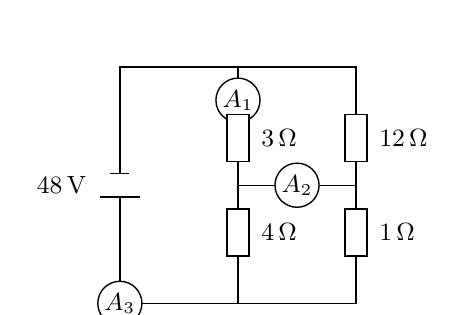
\begin{tikzpicture}[line width=0.5pt]
\draw (0,0)--(0,1.35); \draw (0,1.65)--(0,3)--(3,3)--(3,2.4); \draw (-0.25,1.35)--(0.25,1.35); \draw (-0.12,1.65)--(0.12,1.65);
\node[left] at (-0.3,1.5) {\small $48\,\mathrm{V}$};
\draw (1.5,3)--(1.5,2.72); \draw (1.5,2.44)--(1.5,2.4);
\draw (1.5,1.8)--(1.5,1.2); \draw (1.5,0.6)--(1.5,0)--(0.28,0); \draw (-0.28,0)--(0,0);
\draw (3,1.8)--(3,1.2); \draw (3,0.6)--(3,0)--(1.5,0);
\draw (1.5,1.5)--(1.97,1.5); \draw (2.53,1.5)--(3,1.5);
\draw[fill=white] (1.5,2.58) circle (0.28); \node at (1.5,2.58) {\small $A_1$};
\draw[fill=white] (1.3599999999999999,1.8) rectangle (1.6400000000000001,2.4); \node[right] at (1.67,2.1) {\small $3\,\Omega$};
\draw[fill=white] (1.3599999999999999,0.6000000000000001) rectangle (1.6400000000000001,1.2); \node[right] at (1.67,0.9) {\small $4\,\Omega$};
\draw[fill=white] (2.86,1.8) rectangle (3.14,2.4); \node[right] at (3.17,2.1) {\small $12\,\Omega$};
\draw[fill=white] (2.86,0.6000000000000001) rectangle (3.14,1.2); \node[right] at (3.17,0.9) {\small $1\,\Omega$};
\draw[fill=white] (2.25,1.5) circle (0.28); \node at (2.25,1.5) {\small $A_2$};
\draw[fill=white] (0.0,0.0) circle (0.28); \node at (0.0,0.0) {\small $A_3$};
\end{tikzpicture}\end{center}
\noindent\textbf{33.}\ $A_1$ ampermetrning körsatişini (A) aniqlang.\par
\noindent\textbf{34.}\ $A_2$ ampermetrning körsatişini (A) aniqlang.\par
\noindent\textbf{35.}\ $A_3$ ampermetrning körsatişini (A) aniqlang.\par
\noindent Variantlar: A) 12;\quad B) 7,5;\quad C) 6;\quad D) 3;\quad E) 15;\quad F) 9\par\smallskip
\noindent\colorbox{gray!12}{\parbox{\dimexpr\linewidth-2\fboxsep}{\textbf{Javob: 33--A) 12; 34--F) 9; 35--E) 15}}}\par\smallskip
\noindent\textit{Yechim.}\ Ideal ampermetr $A_2$ ning qarşiligi nol, u köprikning örta nuqtalarini tutaştiradi. Natijada $R_1\parallel R_2$ va $R_3\parallel R_4$ ketma-ket ulanadi:\par
\[R_{12}=\frac{3\cdot12}{15}=2{,}4\ \Omega,\quad R_{34}=\frac{4\cdot1}{5}=0{,}8\ \Omega,\quad I=\frac{48}{3{,}2}=15\ \text{A}\ (A_3).\]
Yuqori qismdagi kuçlaniş $U_{12}=15\cdot2{,}4=36$ V, şuning uçun $I_1=36/3=12$ A ($A_1$). Pastki qismda $U_{34}=12$ V, $I_3=12/4=3$ A. Çap tugun uçun Kirxgof qoidasi: $A_2$ orqali $I_1-I_3=12-3=9$ A oqadi.\par\par\medskip\hrule\medskip
\Needspace{12\baselineskip}\noindent\textbf{36.}\ Qirrasining uzunligi 2 cm bölgan kub şaklidagi 2 ta muz bölagi asosining yuzasi 50 cm$^2$ bölgan, 45,6 g suv quyilgan silindrik idişda taşlandi. $\rho_{muz}=900$ kg/m$^3$.\par
\noindent\hspace*{4mm}a)\ Muzlar erib ketgandan söng suyuqlikning idiş tubiga beradigan bosimini (Pa) toping.\par
\noindent\hspace*{4mm}b)\ Muzlar erib ketgandan söng suyuqlikning idiş tubiga beradigan bosim kuçini (N) hisoblang.\par
\noindent\colorbox{gray!12}{\parbox{\dimexpr\linewidth-2\fboxsep}{\textbf{Javob: a)\ 120;\quad b)\ 0,6}}}\par\smallskip
\noindent\textit{Yechim.}\ Muzlar massasi $m_m=2\cdot0{,}9\cdot2^3=14{,}4$ g, umumiy massa $m=45{,}6+14{,}4=60$ g. Muz erigaç idişdagi suyuqlikning oğirligi töliq tubga tuşadi:\par
\[F=mg=0{,}06\cdot10=0{,}6\ \text{N},\qquad p=\frac{F}{S}=\frac{0{,}6}{50\cdot10^{-4}}=120\ \text{Pa}.\]\par\medskip\hrule\medskip
\Needspace{12\baselineskip}\noindent\textbf{37.}\ Silindrik idişga teng massali suv va kerosin quyildi. Suyuqliklar ustunining umumiy balandligi 27 cm ga teng. $\rho_{kerosin}=800$ kg/m$^3$.\par
\noindent\hspace*{4mm}a)\ Suv ustunining balandligini (cm) aniqlang.\par
\noindent\hspace*{4mm}b)\ Idiş tubidan 8 cm balandlikdagi nuqtada suyuqliklarning hosil qilgan umumiy bosimini (Pa) toping.\par
\noindent\colorbox{gray!12}{\parbox{\dimexpr\linewidth-2\fboxsep}{\textbf{Javob: a)\ 12;\quad b)\ 1600}}}\par\smallskip
\noindent\textit{Yechim.}\ Massalar teng: $\rho_s h_s=\rho_k h_k$, $h_s+h_k=27$ cm. Bundan $h_k=1{,}25h_s$, $2{,}25h_s=27$, $h_s=12$ cm, $h_k=15$ cm. Tubdan 8 cm balandlikdagi nuqta suv içida; uning ustida 4 cm suv va 15 cm kerosin bor:\par
\[p=\rho_k g h_k+\rho_s g\cdot0{,}04=800\cdot10\cdot0{,}15+1000\cdot10\cdot0{,}04=1600\ \text{Pa}.\]\par\medskip\hrule\medskip
\Needspace{12\baselineskip}\noindent\textbf{38.}\ Uzunligi 12 m, qiyalik burçagi $37^\circ$ bölgan silliq qiya tekislik tepasidan 20 kg massali jism sirpanib tuşdi. $\sin37^\circ=0,6$, $\cos37^\circ=0,8$.\par
\noindent\hspace*{4mm}a)\ Jismning qiya tekislik etagidagi tezligini (m/s) toping.\par
\noindent\hspace*{4mm}b)\ Bu jarayonda oğirlik kuçining bajargan işini (J) toping.\par
\noindent\colorbox{gray!12}{\parbox{\dimexpr\linewidth-2\fboxsep}{\textbf{Javob: a)\ 12;\quad b)\ 1440}}}\par\smallskip
\noindent\textit{Yechim.}\ Balandlik $h=l\sin37^\circ=7{,}2$ m. Silliq tekislikda $v=\sqrt{2gh}=\sqrt{144}=12$ m/s. Oğirlik kuçining işi $A=mgh=20\cdot10\cdot7{,}2=1440$ J.\par\par\medskip\hrule\medskip
\Needspace{12\baselineskip}\noindent\textbf{39.}\ Bir atomli ideal gazga 60 J issiqlik berib, hajmi izobarik ravişda 3 marta oşirildi.\par
\noindent\hspace*{4mm}a)\ Bunda gazning absolyut temperaturasi neça marta ortadi?\par
\noindent\hspace*{4mm}b)\ Gazning bajargan işini (J) aniqlang.\par
\noindent\colorbox{gray!12}{\parbox{\dimexpr\linewidth-2\fboxsep}{\textbf{Javob: a)\ 3;\quad b)\ 24}}}\par\smallskip
\noindent\textit{Yechim.}\ Izobarik jarayonda $V/T=\text{const}$, demak harorat ham 3 marta ortadi. Bir atomli gaz uçun $Q=\frac52p\Delta V$, $A=p\Delta V=\frac25Q=24$ J.\par\par\medskip\hrule\medskip
\Needspace{12\baselineskip}\noindent\textbf{40.}\ Issiqlik siğimi 500 J/K bölgan idişda 10 $^\circ$C temperaturali 5 $\ell$ suv bor. Idişga $-5\,^\circ$C temperaturali 1 kg muz taşlandi. $c_{suv}=4200$ J/(kg$\cdot$K), $c_{muz}=2100$ J/(kg$\cdot$K), $\lambda_{muz}=330$ kJ/kg.\par
\noindent\hspace*{4mm}a)\ Natijaviy temperaturani ($^\circ$C) toping.\par
\noindent\hspace*{4mm}b)\ Muzning olgan issiqlik miqdorini (kJ) aniqlang.\par
\noindent\colorbox{gray!12}{\parbox{\dimexpr\linewidth-2\fboxsep}{\textbf{Javob: a)\ 0;\quad b)\ 215}}}\par\smallskip
\noindent\textit{Yechim.}\ Suv va idiş $0\ ^\circ$C gaça soviganda beradigan issiqlik $Q_1=(4200\cdot5+500)\cdot10=215$ kJ. Muzni $0\ ^\circ$C gaça isitişga $2100\cdot1\cdot5=10{,}5$ kJ, töliq eritişga yana $330$ kJ kerak. $10{,}5<215<340{,}5$, demak muzning bir qismi eriydi va $t=0\ ^\circ$C. Muz suv va idiş bergan barça issiqlikni oladi: $215$ kJ.\par\par\medskip\hrule\medskip
\Needspace{12\baselineskip}\noindent\textbf{41.}\ 100 öramli, yuzasi 200 cm$^2$ bölgan töğri burçakli ramka induksiyasi 0,5 T bölgan bir jinsli magnit maydonda induksiya çiziqlariga tik öq atrofida sekundiga 10 marta aylanmoqda. $\pi=3{,}14$.\par
\noindent\hspace*{4mm}a)\ Ramkada hosil böladigan EYuKning amplituda qiymatini (V) toping.\par
\noindent\hspace*{4mm}b)\ EYuKning effektiv qiymatini (V) toping.\par
\noindent\colorbox{gray!12}{\parbox{\dimexpr\linewidth-2\fboxsep}{\textbf{Javob: a)\ 62,8;\quad b)\ 44,41}}}\par\smallskip
\noindent\textit{Yechim.}\ \[\mathcal E_0=NBS\omega=NBS\cdot2\pi n=100\cdot0{,}5\cdot0{,}02\cdot2\cdot3{,}14\cdot10=62{,}8\ \text{V},\]
\[\mathcal E_{ef}=\frac{\mathcal E_0}{\sqrt2}\approx44{,}41\ \text{V}.\]\par\medskip\hrule\medskip
\Needspace{12\baselineskip}\noindent\textbf{42.}\ Gorizontal joylaşgan yassi kondensator qoplamalari orasidagi masofa 1 cm, kuçlaniş 500 V. Kondensator içida massasi $10^{-11}$ kg bölgan zaryadlangan çang zarrasi muallaq turibdi. $g=10$ m/s$^2$.\par
\noindent\hspace*{4mm}a)\ Kondensator içidagi elektr maydon kuçlanganligini (kV/m) toping.\par
\noindent\hspace*{4mm}b)\ Çang zarrasining zaryadini ($10^{-15}$ C) toping.\par
\noindent\colorbox{gray!12}{\parbox{\dimexpr\linewidth-2\fboxsep}{\textbf{Javob: a)\ 50;\quad b)\ 2}}}\par\smallskip
\noindent\textit{Yechim.}\ $E=U/d=500/0{,}01=5\cdot10^4$ V/m $=50$ kV/m. Muvozanat: $qE=mg$,\par
\[q=\frac{mg}{E}=\frac{10^{-11}\cdot10}{5\cdot10^4}=2\cdot10^{-15}\ \text{C}.\]\par\medskip\hrule\medskip
\Needspace{12\baselineskip}\noindent\textbf{43.}\ Suvdagi nurning intensivligi 27 W/m$^2$ ga teng. $c=3\cdot10^8$ m/s.\par
\noindent\hspace*{4mm}a)\ Nurdagi elektromagnit maydon energiyasining ziçligini (J/m$^3$) aniqlang.\par
\noindent\hspace*{4mm}b)\ Nur suvdagi közgudan tik akslansa, közguga beradigan bosimini (Pa) aniqlang.\par
\noindent\colorbox{gray!12}{\parbox{\dimexpr\linewidth-2\fboxsep}{\textbf{Javob: a)\ 1,2$\cdot10^{-7}$;\quad b)\ 2,4$\cdot10^{-7}$}}}\par\smallskip
\noindent\textit{Yechim.}\ Suvda yoruğlik tezligi $v=c/n=3\cdot10^8/(4/3)=2{,}25\cdot10^8$ m/s. Intensivlik $I=wv$:\par
\[w=\frac{I}{v}=\frac{27}{2{,}25\cdot10^8}=1{,}2\cdot10^{-7}\ \text{J/m}^3.\]
Közgudan tik qaytganda bosim $p=2w=2{,}4\cdot10^{-7}$ Pa.\par\par\medskip\hrule\medskip
\Needspace{12\baselineskip}\noindent\textbf{44.}\ Quyoşning diametri $13,8\cdot10^{8}$ m ga, Yer bilan Quyoş orasidagi masofa $1,5\cdot10^{11}$ m ga teng. Fokus masofasi 0,5 m bölgan Yerdagi linza ekranda Quyoşning haqiqiy tasvirini hosil qilmoqda.\par
\noindent\hspace*{4mm}a)\ Tasvir bilan linza orasidagi masofani (mm) toping.\par
\noindent\hspace*{4mm}b)\ Quyoş tasvirining diametrini (mm) toping.\par
\noindent\colorbox{gray!12}{\parbox{\dimexpr\linewidth-2\fboxsep}{\textbf{Javob: a)\ 500;\quad b)\ 4,6}}}\par\smallskip
\noindent\textit{Yechim.}\ Quyoş juda uzoqda, şuning uçun tasvir fokal tekislikda: $f=F=0{,}5$ m $=500$ mm. Tasvir diametri\par
\[d=D\frac{F}{L}=1{,}38\cdot10^9\cdot\frac{0{,}5}{1{,}5\cdot10^{11}}=4{,}6\cdot10^{-3}\ \text{m}=4{,}6\ \text{mm}.\]\par\medskip\hrule\medskip
\Needspace{12\baselineskip}\noindent\textbf{45.}\ Ğalayonlangan vodorod atomining ionlaşiş energiyasi 3,4 eV ga teng.\par
\noindent\hspace*{4mm}a)\ Atom fotonni yutib impuls momentini $2\hbar$ ga oşirsa, uning ionlaniş energiyasi (eV) nimaga teng bölişini aniqlang.\par
\noindent\hspace*{4mm}b)\ Atom fotonni yutib impuls momentini $2\hbar$ ga oşirsa, undagi elektronning orbitadagi tezligi neça marta kamayişini aniqlang.\par
\noindent\colorbox{gray!12}{\parbox{\dimexpr\linewidth-2\fboxsep}{\textbf{Javob: a)\ 0,85;\quad b)\ 2}}}\par\smallskip
\noindent\textit{Yechim.}\ $E_n=13{,}6/n^2=3{,}4$ eV, demak $n=2$. Impuls momenti $L=n\hbar$; $2\hbar$ ga ortsa $n=4$:\par
\[E_4=\frac{13{,}6}{16}=0{,}85\ \text{eV}.\]
Bor modelida $v_n\sim1/n$, şuning uçun tezlik $4/2=2$ marta kamayadi.\par\par\medskip\hrule\medskip
\end{document}